\chapter{\textit{Archipelago}}
The game as it is explained in the following section is the result of the process explained in section \ref{sec:dev}. The rules of the game will be explained before moving on to the final playtest.
 
This playtest was performed at the end of the development and should answer all the questions raised when implementing PCG-based mechanics into hybrid games. Since the game has been thought from the beginning as an experimental concept, it is expected that the answers provided by the different prototypes will transcend the project presented in this paper. This means that the results that will be presented here will contribute to the exploration of making hybrid games in various ways: the successful design choices must be situated in their particular context, to recognize the patterns that support the hybrid nature of the gale; using the same approach, the experimentations that did not provide the expected results will also be analysed.
\section{The Final Prototype}
\label{sec:finalproto}
The first important thing to know about the final version used to playtest is that it was modified in order to cover aspects that were not working as intended. The following section will first present the rules as they were conceived; another paragraph will be dedicated to explain why these final modifications were necessary for the sake of the paper.

\subsection{Setting up the game}
Setting up the board is the beginning of every tabletop game. The board is to be placed on the surface area that the players are using, i.e. a table, and the starting conditions, like the initial resources the players have, will be distributed onto the board. Next step is to assign the player tokens to the respective players. Each player will have their own color on their own "crew tokens" and the color itself is arbitrary, and has no relevant meaning to the game itself, rather than making it easier for the players to know which one is theirs.
When the assigning of the player tokens has been done, and the board has been placed, if the game is played by new players, the next step will be to read through the rules of the game, and to have one of the players read out loud and explain the different phases and the possible actions that can be done, along with the costs and rewards of said actions. If this is not done during the start-up of the game, it can also be done at runtime, as there is no set timer within the application, and the players can take the time they need and refer to the rules.
\subsubsection{The Board}
The following paragraph is a description of the physical board and its components. In figure \ref{fig:compo} are the board used and the tokens the players interact with.
\begin{figure}[!ht]
   \centering
   \begin{subfigure}[b]{\textwidth}
       \includegraphics[width=\textwidth]{Images/Board.png}
       \caption{The board of the final tested version of \textit{Archipelago} explained.}
       \label{fig:boardfinal}
   \end{subfigure}
   \begin{subfigure}[b]{\textwidth}
       \includegraphics[scale=0.65]{Images/tokens.png}
       \caption{The tokens used in the final version of \textit{Archipelago}.}
       \label{fig:tokens}
   \end{subfigure}
   \caption{The analogue components used to play \textit{Archipelago}.}
   \label{fig:compo}
\end{figure}

When starting the game and placing the board, all the players have available 2 \textit{Crew Member}tokens. The \textit{Cargo Hold} contains 4 \textit{Scrap} tokens, and 1 \textit{Alchemy Point}. The castle itself will start off with 3 \textit{Crystal charges} which powers the \textit{Crystal} at level 1. In order to get to level 2, the players will need to acquire another crystal piece. Upgrading the crystal also enlarges the \textit{Cargo Hold}, which can then contain more \textit{Scrap} and \textit{Alchemy Points}.

The \textit{Construction} box is used to place the resources that were spent during the management phase, so they are separated from the \textit{Cargo Hold} - allowing for more clarity when taking decisions. The \textit{Event} box is used to remember which resources are spent during events. 

Finally, the \textit{Allies} box is used to place the \textit{Faction} card of the faction allied with the players. The allied faction being an important parameter in the procedural generation of the events, it was important that players could always remember who they are allied with. 
\subsubsection{The Application}
As the application is started, the players are presented with the layout of the map. In the center is the castle, as is being represented by the physical board on the table. To move around in the world, all that needs to be done, is to click on an island that is within the ring around the castle, which indicates the travel distance possible for the castle each turn. Once an island is clicked on, a travel confirmation dialogue box will appear, and the players will have to confirm that they do indeed wish to travel there.
\subsection{Phase 1 - Castle Management}
\label{sec:p1}
Before the players have to travel around the world within the app, they have the first phase on the board. This phase is called the \textit{Management Phase}. In this management phase, the players can upgrade, repair and expand upon their castle.

\begin{figure}[!ht]
    \centering
    \includegraphics[scale=0.4]{Images/rooms.png}
    \caption{The different types of rooms.}
    \label{fig:roomtype}
\end{figure}

Building a standard room costs 2 \textit{Scrap} tokens, and one \textit{Crew Member} has to be assigned to the construction. This \textit{Crew Member} will not be available during the next phase of the game.
There is no limit for how much players can do during this phase, other than what the players themselves have the resources for. A room can be damaged after an event. In that case, the players flip the room and it is not usable until it is repaired for 1 \textit{Alchemy Point} and 1 \textit{Scrap} per tile occupied by the room. A destroyed room has to be rebuilt from the beginning.

In figure \ref{fig:roomtype} you can see the different rooms available for construction.

During the \textit{Management Phase}, the players can also assign \textit{Crew Members} to a room that is already built. All the rooms have different effects:
\begin{labeling}{\textbf{Mechanic's Workshop}}
\item[\textbf{Mining room}] The crew members assigned to this room will gather \textit{Scrap}. The amount of \textit{Scrap} gathered per \textit{Crew Member} assigned depends on the level of the room.
\item[\textbf{Alchemy Lab}] The \textit{Alchemy Lab} is used on the board to gather \textit{Alchemy Point}. The amount of \textit{Alchemy Points} gathered per \textit{Crew Member} assigned also depends on the level of the room.
\item[\textbf{Mechanic's Workshop}] The \textit{Mechanic's Workshop} is used to repair damaged rooms. When a room is damaged, the players assign 1 \textit{Crew Member} to the mechanic's workshop to repair it. It takes 1 turn per tile occupied by the damaged room to repair it. Upgrading the mechanic's workshop increase the speed at which a room is repaired.
\item[\textbf{Chapel}] The \textit{Chapel} is used to heal \textit{Crew Members} that got injured during an event. It costs one \textit{Alchemy Point} and takes one turn to heal an injury. The number of \textit{Crew Members} that can be healed per turn depends on the size of the \textit{Chapel}.
\end{labeling}

When two rooms of the same type are built next to each other, they can be merged, thus accessing the next level and becoming more powerful (see figure \ref{fig:merge}). Upgrading a room also requires 1 \textit{Alchemy Point} per tile occupied by the upgraded room. Again, this will require a player to temporarily set a crew inactive, as it has to build the room. It is worth noticing that the crystal as to be upgraded in order to merge rooms.

\begin{figure}[!ht]
    \centering
    \includegraphics[scale=0.4]{Images/merge.png}
    \caption{The room merging system. In the top left corner of each tile, the players can see the \textit{Crystal}'s level required to build the room.} 
    \label{fig:merge}
\end{figure}
\subsubsection{Collaboration and Mastery}
The merging mechanic introduces specialization or \textit{Mastery}. In \textit{Archipelago}, all players can perform almost all the basic actions in the game. There is no specific skill related to a specific role. However, a player alone cannot perform all the actions required by the game at the same time: the amount of actions that a player can perform is directly related to the number of \textit{Crew Members} that this player commands. Therefore, it is important to encourage the players to split the tasks among them. The tasks can be divided into several groups that are related to the type of rooms that can be built in the castle. When a players spends one of her \textit{Crew Member} to merge a room, that player gain a \textit{Specialization token} of the same type as the room that was upgraded. There are different types of \textit{Specialization Token}, depending on size of the room that has been upgraded after merging (see figure \ref{fig:spec}). 

\begin{figure}[!ht]
    \centering
    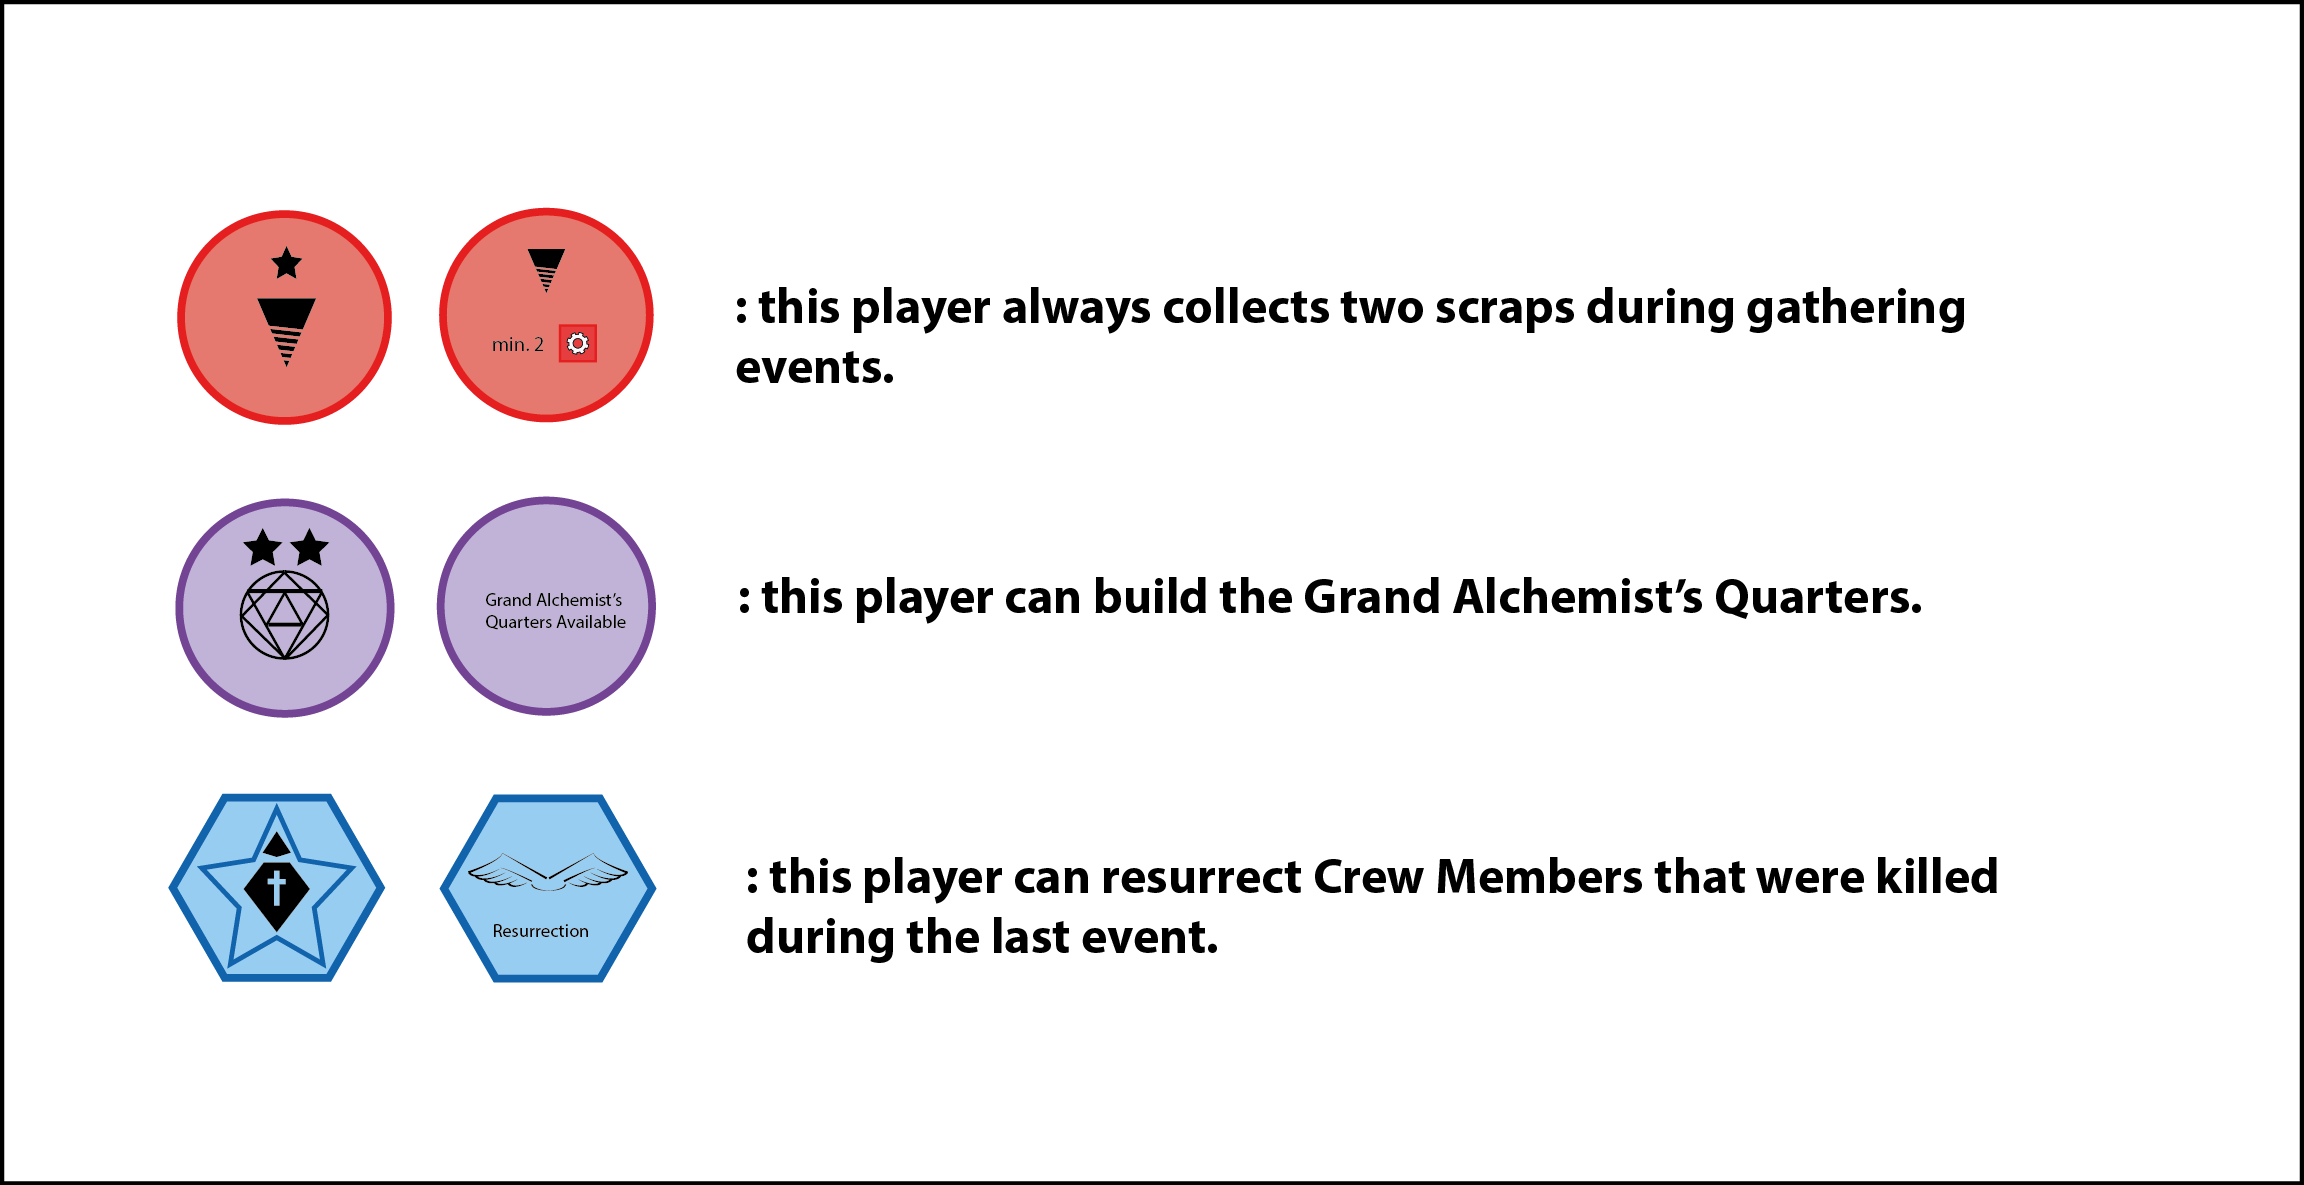
\includegraphics[width=\textwidth]{Images/Specialization.png}
    \caption{Examples of specialization tokens that players can have. Each of the tokens represents a bonus that can be useful when performing the procedurally generated events.}
    \label{fig:spec}
\end{figure}

The first type of \textit{Specialization token} grants a small bonus when visiting an island. The second type of \textit{Specialization token} always allow the player who has it to build the biggest rooms, called \textit{Mastery Rooms}. They take four construction spaces and grant the player the \textit{Mastery token} (see figure \ref{fig:temp}. This token provides important bonuses that affect the outcomes of the event.
 
\begin{figure}[!ht]
    \centering
    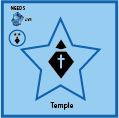
\includegraphics[scale=1]{Images/mastery.png}
    \caption{The Temple, that provides the priest's \textit{Mastery} token. This token allows the player to resurrect \textit{Crew Members} that died during an event for 1 \textit{Alchemy Point}.}
    \label{fig:temp}
\end{figure}

The bonus provided by the \textit{Mastery token} are very important, and the game can hardly be finished without them.

It is important to notice that the \textit{Specialization} tokens are only attributed to the first player who merges rooms of the same type. 
\subsection{Phase 2 - Exploring the World}
\label{sec:p2}
When the first phase is over, and all the crew tokens have been assigned, the next phase is to explore the Archipelago.
As mentioned before, the first thing the players have to do in the world map, is to click on the reachable island they want to travel to. Once they have accepted to travel there, and have reached the location, the players will have to select a \textit{location} that they would like to explore.
Each area are connected to a type of resource, either it is a gathering area which will mainly yield building materials, or it is the research area which will yield mainly alchemy points. The players talk amongst themselves which one they would like to explore, and will have to choose based on what their current needs are. Once a location has been selected, the players will be presented with the event.

The player who is currently controlling the application reads out the event along with the possible options. It is now up to the players to talk amongst themselves to figure out which option they would like to pick. They also must decide which player should send a \textit{Crew Member}, according to which player is specialized. Also, the players have to remember that a \textit{Crew Member} can die in the process. The first class option is usually just sending a member of the crew down to complete the event, but there can be other options as well. The second class option adds a resource to the condition. It can be any of the four resources used in the game. The third class option requires a specialization token. In this case, it is the player that has the token that must send one of her \textit{Crew Member}. 

After the players have reached their conclusion and selected their option, the application will present them with the resulting outcomes of the event. It might be that they have lost a player token, gained one, a room has been destroyed, or simply that they got some resources. The outcomes vary. When the players have received their rewards and applied the results to the board, the players go back to the \textit{Management Phase}.

\subsection{Clean-up and start a new turn}
When returning from an event, all the pieces that were used the previous round, i.e. the crew tokens used for construction, the tokens assigned to the rooms, and the tokens used in the events, are returned to the players, and the board is cleaned up.
If an event yielded too much resources so that the cargo hold of the castle would be overfilled, it is up to the players to discuss which they would like to keep, and which to discard, before going back to phase 1 - management.
When this is done, the game repeats as described above with phase 1 and 2 and back again.

\subsection{Special Events}

Somewhere along the game, the players will most likely encounter the \textit{Special Events}. There are as of right now, two types of special events.

The first type is the fighting event. When this event occurs, the players will be presented with a scenario where two of the factions within the game, are fighting each other. It is then up to the players to decide whether they want to leave them alone, or if they would like to assist them. If they want to assist them, they have to choose their side. If the players are already friendly with one of the factions, they might want to assist that faction again. This choice is completely up to the players.

The other event type is memory based. It is an event that is based on previous events that the players have completed. The event is special in that it is based on previous data. If the players visited an island controlled by the Highbournes, and they used some special healing on one of the options, then the special event could say something like "The highbournes saw you at the island, and want to learn how to use your healing magic". It is then up to the players to decide whether or not they want to help them, or not. Keeping in mind that their current standing with the faction will influence the outcome of whatever option they choose. 

\subsection{Reaching the end - Winning condition}
At one specific point on the map, there is a goal island. This island is the one the arrow is pointing towards, and is the one that the players are supposed to head towards in order to complete the game, and win.
If the players are able to reach this island, the game is over. The players will be presented with an ending screen in the application, and then they can choose to start a new game if they so choose. 

\subsection{Losing the game - Losing conditions}
There are a number of different ways to lose the game. Since it is a collaborative game, if one of the players manages to get all his or her crew tokens killed, the game is over. Every player must have at least one crew token, in order for the game to still be in play.
Should the castle run out of crystal charges, the game will be over as well, as this would mean that the castle would be stuck floating in space and not be able to move.

\section{Last Playtest}
The prototype described above is the last one that was built during this prototype. It is the result of the combination of the game mechanics created for the purpose of experimenting hybrid games and the implementation of PCG to create a new kind of play experience.
\subsection{Modifications for testing purposes}
Earlier prototypes showed that the game was not ready to provide relevant results about its experimental purpose. Therefore it was decided to alter the prototypes with a few modifications in order to obtain the necessary results. The players were not aware of the modifications.

\subsubsection{Map layout}
Originally, the map should have introduced a mechanic based on \textit{interest points}. The players should not have to only reach the final island on the map to win the game, but explore the Archipelago in order to find three specific islands before going to the final island. The islands should have been possible to localise thanks to clues gained in some special events. The intermediary islands would then only be revealed when the players would be close enough (if the island is within the circle showing the range of the next move). First, the provided clues should have been visual, and thus recognizable thanks to a variety of graphical assets, which were not ready when the game needed to be tested.

It was decided to simulate it by indicating the next island to reach thanks to the arrow. The arrow only showed a general direction where the island was, and would be revealed with a halo of another colour as the one used for the other islands when the players would be close enough. This would not perfectly reproduce the intended experience, but at least it would simulate the feeling of exploration by trying to find the correct island among others. This difference between the intended experience and the one simulated by the prototype was of course taken into account when analysing the results.
\subsubsection{Special events occurrences}
The special events were a difficult part of the design of the game. It was necessary to have them occurring not too often, so they would always be unpredictable for the players. This is also why they have such particular parameters to be triggered. However, internal tests performed before the final playtest with players showed that the events were not occurring often enough. 

Since analysing the reaction of the players when facing a special event, it was decided that some regular events would be pre-made and set to occur at a given turn. To do so, the island would also be set to only generate one location during this turn. Also, two out of the three options offered in the event included in that location would trigger a special event, which would ensure that the players would have to go through it before moving on to the next island. The special events were set to be triggered at least once between each intermediary islands.
\subsubsection{Progression and risk}
Since the special events are a way to increase the risk, and so the difficulty of the game, the problem of the special events not being triggered often enough generated a problem in the game's progressive difficulty. It happened that the layers would literally have very few difficulties progressing through the game, because the risk was not increasing fast enough. To solve this problem, the risk parameter was set to be also altered every time the players would reach an intermediary island.

This altered the experimental purpose of the game, because the difficulty was supposed to naturally increase with the player's progression. However, it was necessary to have more control over the difficulty so that the final prototype could offer more relevant results about the play experience itself, and not only the technical data about the generation of content.

\subsubsection{Using a portable device}
After these modifications, the application was ready to provide relevant data. However, there was a last problem that would alter the data too much to be ignored. This experiment was supposed to test hybrid games as tabletop games using a digital component to enhance its gameplay. Throughout the development of the game, the application was running on a Personal Computer during playtests. It was important for the final playtest to be able to use a smartphone or a tablet as a digital component. This would allow us to gather data of better quality about how intrusive the digital component is in the flow of hybrid games.  
\subsection{Material, Scope and resolution}
The \textbf{Material} of the prototype was closer of what players would expect when playing a hybrid game. It was the first time that the game was tested with analogue components using other material than paper, thus changing the tactility of the different pieces. With earlier prototypes using paper to iterate more quickly, the players had shown frustration when not being able to pick up the bits of paper, or losing them. Using other material than paper for the tokens would ensure that this problem would not alter the results. As explained above, the digital component was a tablet for the first time. This would help providing the necessary information related to the flow of the game. However, since the port to tablet was made in a very brief time, some problems with zooming as well as fluidity drops when moving the camera around on the map would alter the experience. This problem was explained to the players prior to testing, and taken into account in the final results.

The 

This is the highest fidelity prototype that was created during this project. Although all the visual assets are still place-holders, the prototype uses a tablet as a digital device and that all the mechanics are implemented. 
\subsection{The Playtest}
\subsection{Questionnaire}

\section{Results and Data Analysis}
\subsubsection{Classifying data}
\subsubsection{Interpreting Data}